% !TEX program = lualatex
\documentclass[11pt]{article}

% -------- LuaLaTeX : polices et langue --------
\usepackage{fontspec}
\setmainfont{Latin Modern Roman}
\setsansfont{Tex Gyre Heros}
%\renewcommand{\familydefault}{\sfdefault} % force le sans serif par défaut
\usepackage{polyglossia}
\setdefaultlanguage{french}

% -------- Mise en page --------
\usepackage[a4paper,margin=1cm]{geometry}
\usepackage{multicol}
\usepackage{fancyhdr}
\pagestyle{empty}
\usepackage[most]{tcolorbox}

% -------- Mathématiques --------
\usepackage{amsmath,amssymb,mathtools}
% \usepackage{siunitx}
% \sisetup{locale=FR}

\usepackage{enumitem}
\setlist[itemize]{left=0pt}
\setlist[enumerate]{left=0pt, label=\textbf{\arabic*}.}

\usepackage{ProfCollege}
\usepackage{ProfMaquette}

\usepackage{tabularray}

% -------- Divers --------
\setlength{\parindent}{0pt}

\begin{document}

\begin{multicols}{2}

\begin{Maquette}[Fiche]{Theme=Arithmétique, Niveau=Quatrième}

\begin{exercice}
    Dans un collège, il y a $162$ élèves en classe de troisième.
    \begin{enumerate}
        \item Combien peut-on former d’équipes de basket de cinq joueurs ? Combien d’élèves restera-t-il ? 
        \item Combien peut-on former d’équipes de football de onze joueurs ? Pour compléter la dernière équipe, on fait appel à des élèves de quatrième, combien en faut-il ?
    \end{enumerate}
\end{exercice}

\begin{exercice}
    Complète la grille de mots croisés suivante.
    \begin{enumerate}
        \item $3$ dans la division euclidienne de $67$ par $22$.
        \item $12$ est un … de $36$.
        \item $25$ ou $8$ dans $25 \times 8 = 200$.
        \item Nombre qui est divisé dans une division.
        \item $3$ dans la division de $31$ par $7$.
        \item $27$ ou $12$ dans $27 + 12 = 39$.
    \end{enumerate}
    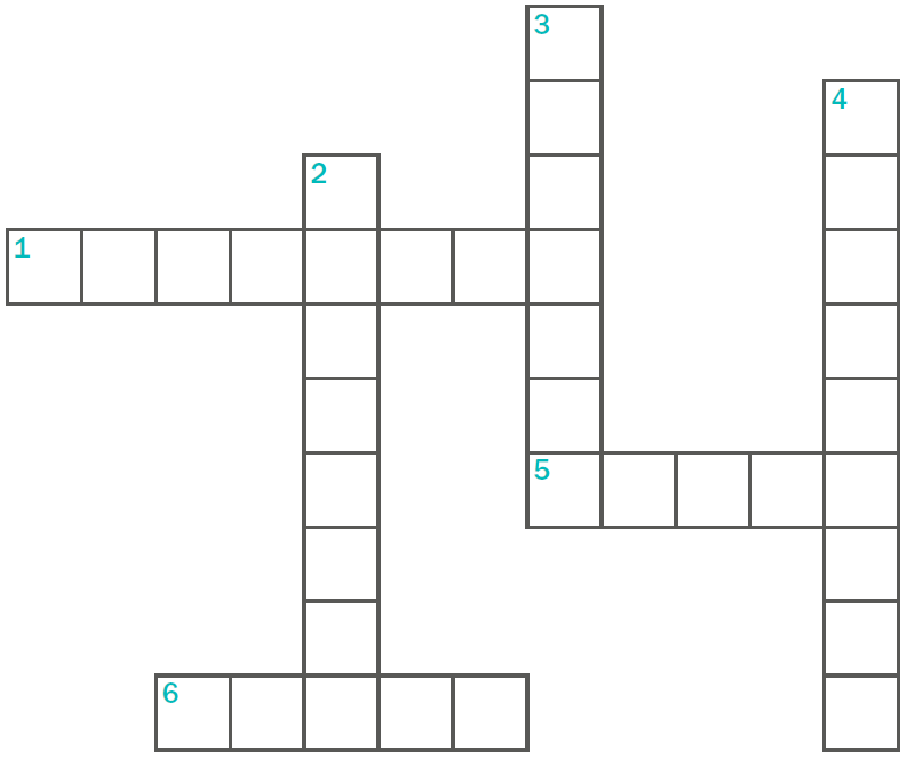
\includegraphics[width=\linewidth]{Images/MotsCroises.png}

\end{exercice}

\begin{exercice}
    À la consigne « Écris la division euclidienne de $68$ par $11$ », un élève a répondu : $68 = (11 \times 5) + 13$.
    \begin{enumerate}
        \item Pourquoi est-ce faux ?
        \item Donne la bonne réponse.
    \end{enumerate}
\end{exercice}

\columnbreak 

\begin{exercice}[Source=DNB Juin 2024 Centres étrangers]
    Un entraîneur de sport prépare deux circuits d’entraînement contenant plusieurs exercices de cardio et de renforcement musculaire :
    \begin{itemize}
        \item un circuit commence à l’exercice 1 et se termine en revenant à l’exercice 1 ;
        \item le circuit 1 contient cinq exercices. Chaque exercice dure 40 secondes et doit être suivi de 16 secondes de repos permettant de se rendre à l’exercice suivant ;
        \item le circuit 2 contient dix exercices. Chaque exercice dure 30 secondes et doit être suivi de 5 secondes de repos permettant de se rendre à l’exercice suivant.
    \end{itemize}
    \begin{center}
        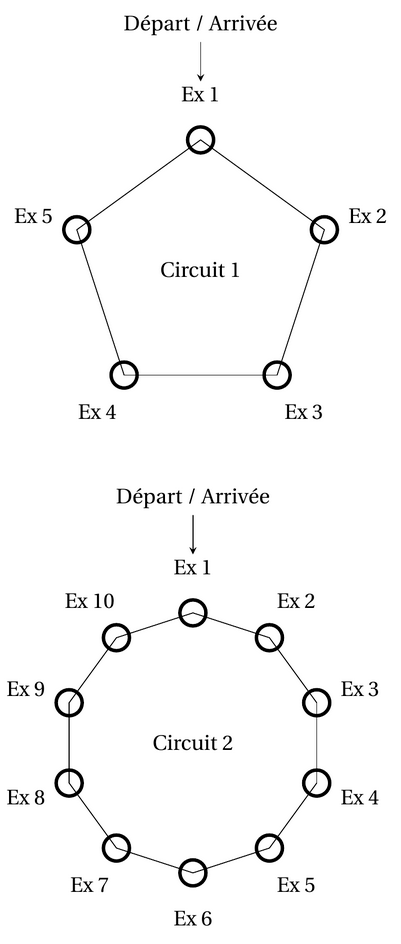
\includegraphics[width=0.65\linewidth]{Images/Parcours.png}
    \end{center}
    \begin{enumerate}
        \item Montrer que le circuit 1 s’effectue en 280 secondes et que le circuit 2 s’effectue en 350
secondes.
        \item Une séance d’entraînement est constituée de plusieurs tours du même circuit. Au coup de sifflet de l’entraîneur, Camille commence une séance d’entraînement sur le circuit 1 et Dominique sur le circuit 2.Combien de temps faut-il à Camille et Dominique pour se retrouver en même temps pour la première fois au départ de leur circuit ? Exprimer cette durée en minute et seconde.
    \end{enumerate}
\end{exercice}

\columnbreak

\begin{exercice}[Titre=Jeu de Juniper Green]
    Version à deux joueurs :
    \begin{itemize}
        \item le joueur qui commence barre un nombre pair
        \item ensuite chaque joueur doit barrer un nombre (pas encore barré) qui est un multiple ou un diviseur du nombre barré par son adversaire
        \item si un joueur ne peut barrer aucun nombre, la partie s’arrête et il a perdu
    \end{itemize}

    \begin{center}
    \begin{tblr}{
            colspec={c c c c}, 
            hlines, vlines,
            abovesep=3pt, % espace au-dessus
            belowsep=3pt  % espace en-dessous
            }
            1 & 2 & 3 & 4 \\
            5 & 6 & 7 & 8 \\
            9 & 10 & 11 & 12 \\
            13 & 14 & 15 & 16 \\
        \end{tblr}
    \end{center}
\end{exercice}

\begin{exercice}[Titre=Jeu de Juniper Green]
    Version à un joueur : l’objectif est de barrer le plus de nombres à la suite en respectant la règle « multipe ou diviseur du nombre précédent ».\\
    On enlève la contrainte de commencer par un nombre pair.\\
    Avec les nombres de $1$ à $16$, on peut trouver une liste maximale de $14$ nombres.
\end{exercice}

\begin{exercice}[Calculatrice=false]
    Complète avec les croix nécessaires.

    \vspace{1.1em}
    \begin{tblr}{
            width=\linewidth, % occupe toute la largeur
            colspec={c X[c] X[c] X[c] X[c] X[c]}, % colonnes extensibles
            hlines, vlines,
            row{1} = {font=\bfseries}, % première ligne en gras
            abovesep=3pt, % espace au-dessus
            belowsep=3pt  % espace en-dessous
            }
            est divisible par & 2 & 3 & 5 & 9 & 10 \\
            570 &   &   &   &   &   \\
            640 &   &   &   &   &   \\
            951 &   &   &   &   &   \\
            612 &   &   &   &   &   \\
            225 &   &   &   &   &   \\
            576 &   &   &   &   &   \\
            757 &   &   &   &   &   \\
        \end{tblr}

    \vspace{1.2em}
    Par quelle expression aurait-on pu remplacer « est divisible par » ?
    
\end{exercice}

\columnbreak

\begin{exercice}
    Voici une manière d’illustrer les diviseurs du nombre 20 :

    \begin{center}
        \Decomposition[Poisson, CouleurPoisson=Cornsilk]{20}    
    \end{center}
    
    Complète.
    \begin{itemize}[label={}]
        \item \Decomposition[Poisson, CouleurPoisson=Cornsilk, ElementsVisibles={1,3,6,12}]{24}
        \item \Decomposition[Poisson, CouleurPoisson=Cornsilk, ElementsVisibles={3,15}]{30}
        \item \Decomposition[Poisson, CouleurPoisson=Cornsilk, ElementsVisibles={8}]{16}
        \item \Decomposition[Poisson, CouleurPoisson=Cornsilk, ElementsVisibles={5}]{90}
        \item \Decomposition[Poisson, CouleurPoisson=Cornsilk, ElementsVisibles={20}]{60}
    \end{itemize}
    Dessine les schémas pour les nombres $17$ et $31$.
\end{exercice}

\columnbreak
\begin{exercice}
    Trouve un chemin permettant de relier les deux super-héros en ne passant que par des nombres premiers. (pas de passage en diagonale)
    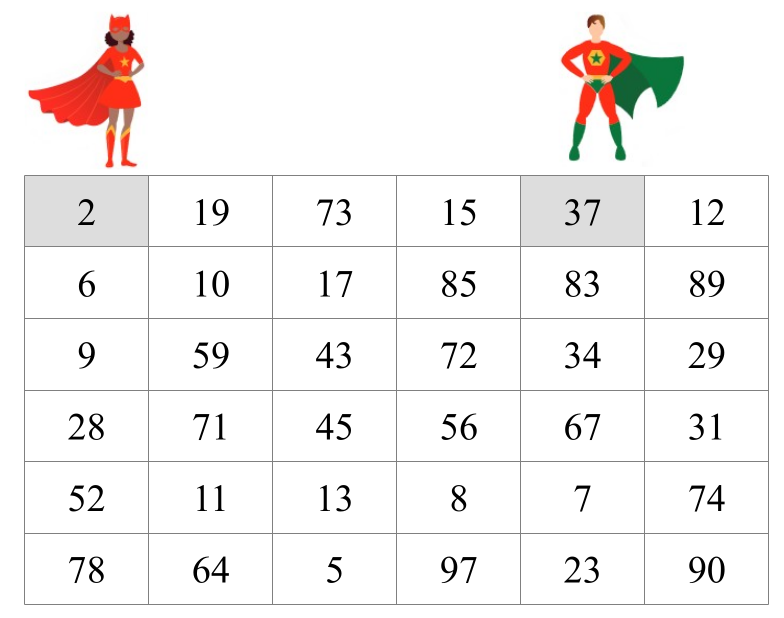
\includegraphics[width=\linewidth]{Images/Labyrinthe.png}
\end{exercice}

\end{Maquette}

\end{multicols}

\end{document}
